\chapter{Introduction}
The robotic field has experimented an enormous increase in the past years. 
Different components and systems have improved.
As an example, cameras have evolved and low-cost 3D sensors have appeared. 
This fact provides a higher and more reliable amount of information for the computer vision system of the robot.  
Also, the processing units have been upgraded, allowing a larger amount of computing that permits the inclusion of more complex algorithms in these robots.  
% Different aspects of the robots has improved such as the sensors or actuators being integrated. 
% The processing and analysis of external data has been also upgraded. 
This leads to the increasing introduction of robots in human environments with assistive or social tasks. 
\\


The first automatisms performed their tasks without being aware of their environment. 
Their work area consisted mainly on closed areas in to which humans were denied entry. 
But the introduction of robots in the houses and other places frequented by humans increases the importance of perceiving the environment accurately. 
% The integration of robots in areas inhabited with humans increase the importance of the environment perception. 
The robot must be able to recognize and interact with the objects and persons around it. 
This interaction needs many different sensors or input systems and as many output systems to retrieve the information and respond to it correctly.  
\\

% Humans are a key part in that interaction. 
% Social and assistive robots are designed to help humans in their everyday life. 
% To this purpose, the robot should be able to recognize gestures or poses of the users or actions they are performing in order to infer what they are feeling or what they need. 
% As an example, if the user has fallen, the robot should recognize the pose to deduce the user's status. 
% Afterwards, it might be able to conclude that the user needs help from him in order to get up. 
% Finally the robot might offer a support or even help the user in the standing up action. 
% \\

The human environment has a lot of variables that contain information about the user's intentions or actions. 
One of this variables are the objects the human uses. 
For example, if a person is holding a toothbrush, he is probably going to brush his teeth. 
Also, if the user is holding the keys in his hand he might be going out of the house. 
It can be easily seen that identifying the objects the humans hold in their hands, key information about the actions they are undergoing is extracted. 
If the robots could recognize those objects, they could adapt their behaviour to the situation around them. 
As an example, if the user is holding a book, he is probably reading and  he does not want to be disturbed except for an emergency. 
The robot could then change its behaviour to the new constrains of the environment, for example, making as less noise as possible. 
\\

Having a system that could track and identify in-hand objects could improve the robot's interaction with its environment.
For this purpose I have developed a system that is able to learn and recognize hand-held objects in real time through a simple and intuitive gesture interface. 
This software is capable of recognizing the user's skeleton and, from it, extract the hands position. 
With this information the system studies the area around the hands and compares it with a previously acquired dataset.
It is possible to use the software without input and output devices such a screen or a mouse, since it integrates a pose interface. 
This fact easies the transition from the dataset acquisition to the recognition of objects and allows the system to be implemented in a robot. 



% Robots are being increasingly introduced in human envionments. 
% Social and assistive robot's behaviour depend on the actions of the individuals around it. 
% Some of those actions may be inferred fro the object the user is holding. 
% For exmple, if a human is holding his keys, he is likely to go out. 
% An assistive robot for visually impaired people may respond to this action by handing him over his cane. 
% Recognizing the object the user is holding may help the robot to understand better the situation, improving the human-robot interaction. 
% For this purpose I have developed a system that is able to learn and recognize hand-held objects in real time through a simple and intuitive gesture interface. 

% \newpage 
%\addcontentsline{toc}{chapter}{Socio-economical context}
\section{Socio-economical context}
\label{context}
Europe's population is ageing.
This phenomena occurs because of the augment in the live expectancy and the declining of birth rates. 
Recent studies provided by the World Health Organization (WHO) showed that the live expectancy in Spain is the highest in Europe, specially in women \cite{who_live_expectancy}.
Spanish women live an average of  85.1 years in 2012, and the men around 79 years. 
In fact, the Spanish women live expectancy is only behind the Japanese women, that is, the second highest level in the world. 
\\

In the World Population Ageing Report of 2013 it is stated that "by 2050, Bosnia and
Herzegovina, Germany, Malta, Portugal, Serbia and Spain are projected to attain median ages of
50 years or more"\cite{world_population_ageing}. 
This means that soon enough there are going to be more elder people than young people. 
How are we going to be able to support and aid that major sector of the population?
The solution might be to incorporate robots to help in this task. 
\\

Assistive robots can help elder people to interact with their environment. 
They can cooperate in the health control of the user testing the blood pressure or recognizing falls. 
Also, social robots may maintain a conversation and interact with people, for example, reminding them to take a specific medication. 
Japan is the country with the highest population ageing of the world. 
This country is the world leader in the assistive robotics field. 
Recently the he International Organization for Standardization (ISO) has adopted Japanese standards for assistive robotics technology \cite{japan1}\cite{japan2}.
The Japanese government is studying to introduce a system of assistive technologies and hence the funding in this field is high. 
As an example of the technology being developed in this country, the Pepper assistive robot was recently anounced by SoftBank Corp\cite{cheap_humanoid}.
It is a robot that costs less than two thousand USD and that is capable of maintaining a conversation with the user. 
Pepper is not capable nowadays of performing assistive tasks. 
It has a humanoid form with arms, but they are only used to express and empathize the information that it is giving. 
Is hence the first step towards more environment-aware and interactive low-cost robotics.
% Is humanoid and has arms, but at least until now they are only used to express and empathize its words.  
\\

In Spain the assistive field is mainly being evolved in universities and investigation groups. 
Projects such as the RobAlz between the Fundación Alzheimer España (FAE) and the Carlos III University \cite{robalz} are developed to improve the interaction between robots and, in this particular case, Alzheimer patients.  
Another example of the Spanish investigation in the field is the work performed by the Ave María Foundation \cite{assistive_spain}.
They have introduced various robots in the therapies of their patients. 
Nao is a small robot that can recognize faces, sounds and is able to walk. 
It is used to instruct therapy seasons. 
Another one is the robot REEM, which is more than 1.6 m height. 
It is used to transport the necessary items such as clothes or food around the place, allowing the employees to center in assistive tasks. 



% In the past seven years the world has experienced the effects of the recession that appeared in the late 2000s decade. It still affects the economy nowadays and the experts do not know how many more years the situation will stay the same. \\

% In Spain the recession has had a big impact that can still be seen in the unemployment numbers and jobs offers. Also, the poverty has increased enormously and the quality of life has decreased together with the salaries.  
% \\

% There is a general discontent with the politics and the banks. Pessimism is everywhere, as well as the feeling that it is needed a change of direction in both fields. 
% \\


% This economic context has created and motivated new ways of investigating and living, always aiming at spending as less as possible. It has triggered a change in the perception of the knowledge and whether it should be restricted using patents or not. Most of the scientific community now supports the open source initiative, a fact that has increased the rapidity of the new discoveries and technology improvements. 

% \begin{figure}[h]
% 	\begin{center}
%     
\includegraphics[scale=0.3]{img/intro/osi.eps}
% 	\caption[Open Source Initiative Logo]{Open Source Initiative Logo}
% 	\end{center}
% \end{figure}


% The idea of creating common software, of aiding other investigators to easily replicate the work already done and continue from that point instead of "reinventing the wheel" started in the past century. In 1998 the Open Source Initiative (OSI)\cite{osi} was formed, and its definition is recognized as the standard. According to them, "Open source does not just mean access to the source code. The distribution terms of open-source software must comply with the following criteria: Free Redistribution, Source Code, Derived Works, Integrity of The Author's Source Code, No Discrimination Against Persons or Groups, No Discrimination Against Fields of Endeavor, Distribution of License, License Must Not Be Specific to a Product, License Must Not Restrict Other Software,  License Must Be Technology-Neutral"\cite{osi_def}. 
% \\

% Open Source is crucial in the development of new knowledge and not only in the Software field, but in all the science and technical disciplines. 




%\addcontentsline{toc}{chapter}{Motivation}
\chapter{Motivation}

Robotics is a field that is experiencing a huge impulse currently. And more specifically, Open Source robotics is growing rapidly. 
\\

The idea of creating common software, of aiding other investigators to easily replicate the work already done and continue from that point instead of "reinventing the wheel" started in the past century. In 1998 the Open Source Initiative (OSI)\cite{osi} was formed, and its definition is recognized as the standard. According to them, "Open source does not just mean access to the source code. The distribution terms of open-source software must comply with the following criteria: Free Redistribution, Source Code, Derived Works, Integrity of The Author's Source Code, No Discrimination Against Persons or Groups, No Discrimination Against Fields of Endeavor, Distribution of License, License Must Not Be Specific to a Product, License Must Not Restrict Other Software,  License Must Be Technology-Neutral"\cite{osi_def}. 
\\

It is my believe that Open Source is critical in the development of new knowledge and not only in the Software field, but in all the science and technical disciplines. This is how the idea of increasing that common pool of tools with another one that might be useful appeared. 
\\
\begin{wrapfigure}{r}{0.3\textwidth}
	\centering
    
\includegraphics[width=0.25\textwidth]{img/intro/open_source.eps}
	\caption[Open Source Initiative Logo]{Open Source Initiative Logo}
\end{wrapfigure}

It is noticeable the mark that Open Source has throughout the project. From the libraries being used in it to the Robotic Operating System of which this project is but another package. All of them are Open Source. Also, the tutorials, examples and different web-pages with useful comments and aids for those who are learning has been critical in this project's development. Nothing of this could have been possible without the idea of Open Source code. 
\\

Apart from the want of making useful Open Source code, there remain another motivation unexplained. That is, the specific subject of this project. 
\\

Previously, I have developed other projects involving designing and constructing wheeled robots. It was then the idea of creating different packages that glued together could suit almost every robot appeared. One of the most interesting fields that can be used in virtually all types of robots is Computer Vision. 
\\

Computer vision has experience an important improvement in the last years through the upgrade of the hardware and software that compose it. The hardware such as acquisition elements (cameras, depth sensors, etc) and computing elements (PCs or other programmable devices) have experienced a rapid advance in the past years. It allowed to process more data that is now obtained more accurately and with less noise. This increase in the computing power of the equipment created a possibility of introducing more complex libraries and frameworks and even operating systems. 
\\

But Computer Vision is an ample area, why choosing object recognition? The project being developed is intended to be useful, not just a mere hobby. It occurred to me that apart from being useful in the interaction with robots and cognitive robots more particularly, this software could be used with visually impaired people, as an example. Mainly, with people that had a sudden loss of vision and that is not used to detect the objects by its shape, or cannot differentiate them by the contour. 


\section{Proposed solution for in-hand object recognition: \\OCULAR}

In this thesis a software has been developed that is intended to be used in assistive and social robots.
The name and the logo (figure \ref{ocular_logo}) of the project gives a first idea of the system's goal. 
The name of the project, OCULAR, is an acronym of "On-line objeCt Learning And Recognition". 
The first word, on-line, refers to the fact that the learning of new objects is done in real time. % there is no need of a training phase in which the software is not operative. 
Figure \ref{ocular_logo} presents the logo of the software, which gives two additional pieces of information: 
the object learning and recognition is performed in-hand and the input of the system is a RGB-D (Red, Green, Blue and Depth) sensor, such as a Kinect. 
This type of sensor provides 2D and 3D information of the user located in front of it. 

\\

\begin{figure}[H]
	\begin{center}
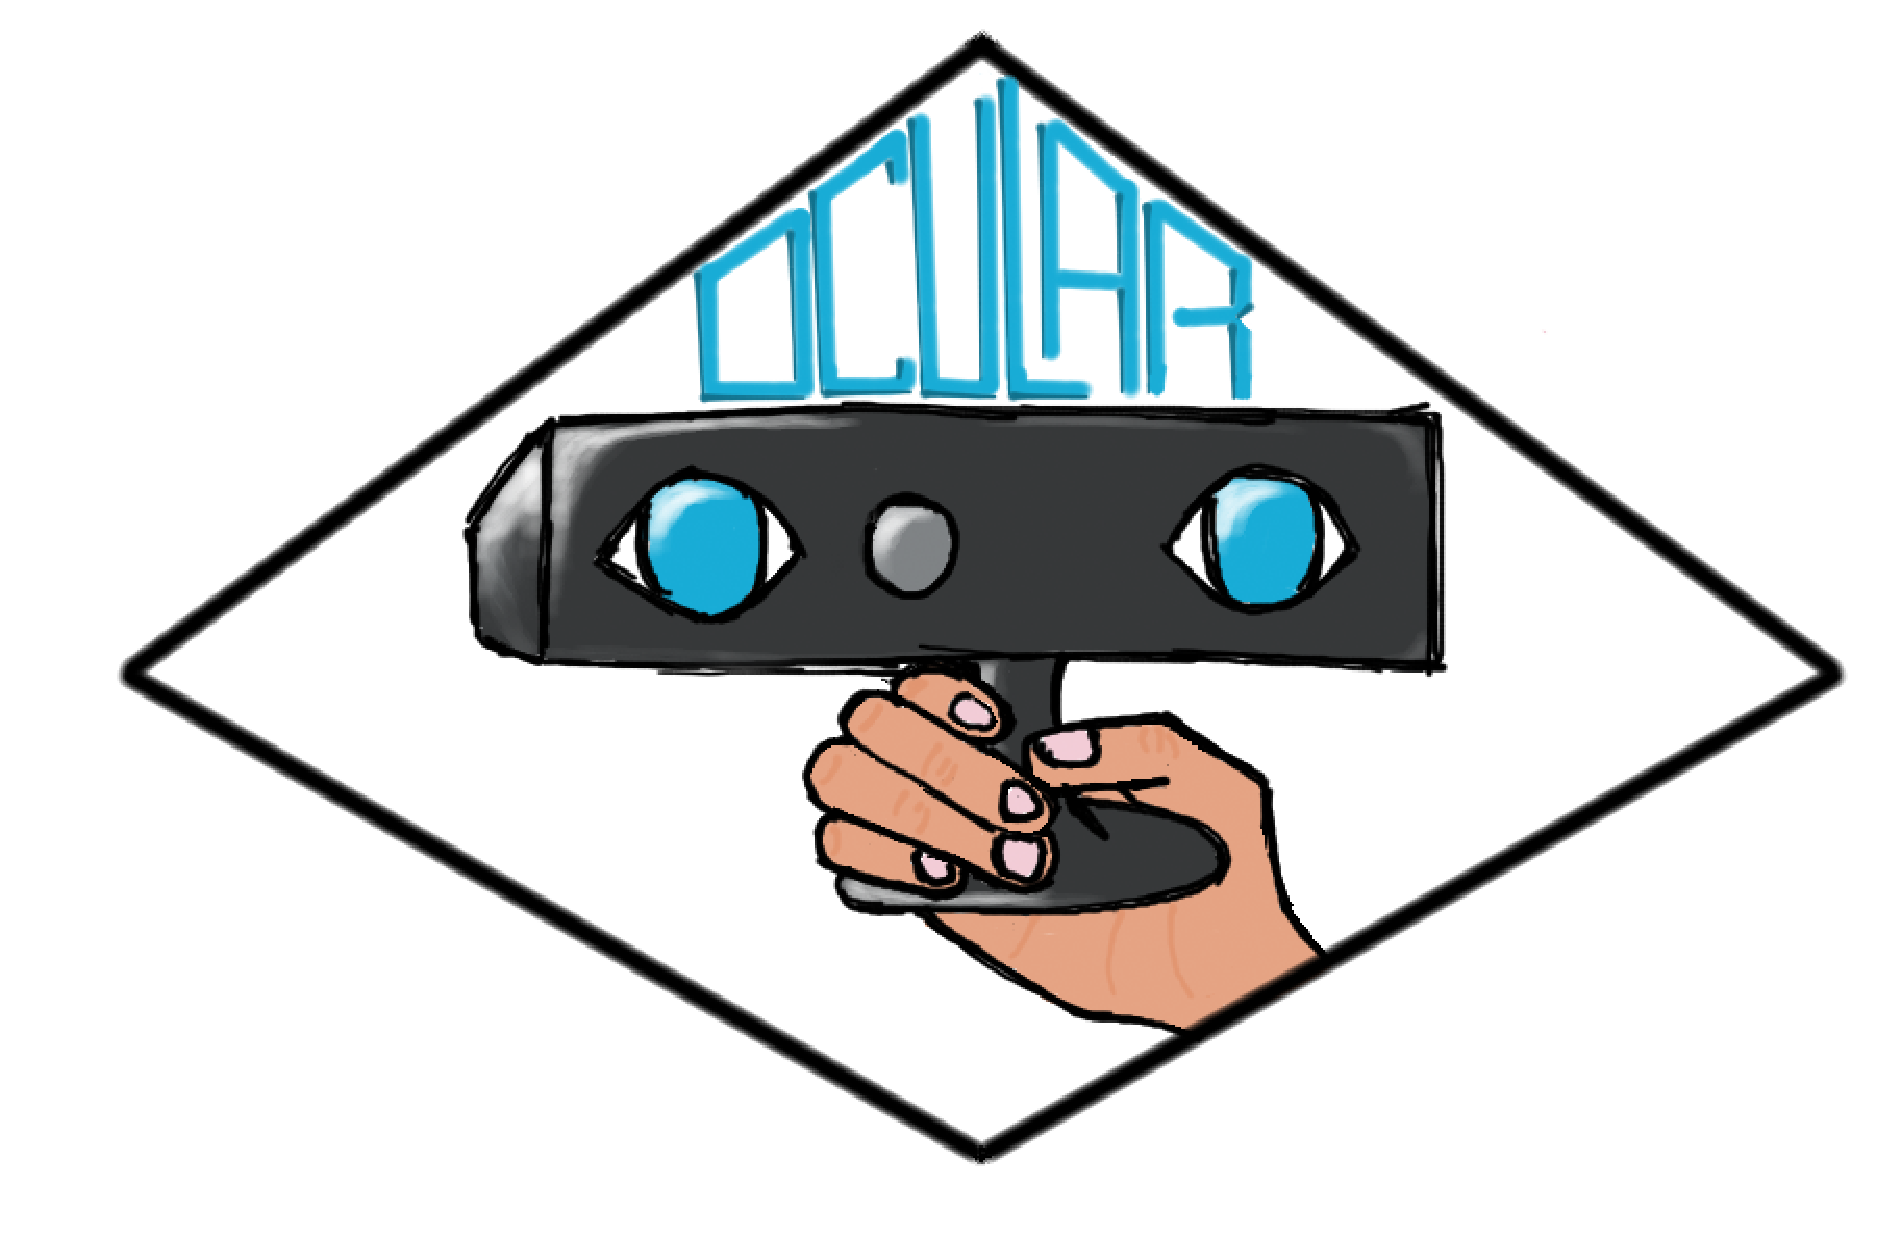
\includegraphics[scale=0.3]{img/ocular_logo.eps}
	\caption[OCULAR Logo]{OCULAR logo}
		\label{ocular_logo}
	\end{center}
\end{figure}

Since it is intended to be running on a robot, the software has to implement an intuitive human-machine interface. 
A gestural interface was designed that allows the passing of information from human to computer in a simple way. 
The software has two differentiated modes, the learning or data acquisition mode and the recognition or system exploitation modes. 
The system is able to detect the change of the mode using the pose of the user as can be seen in figures \ref{learn} and \ref{recognize}. 
% The usability of the software is fully dependent on the easy transition for the user from one mode to the other. 
% Furthermore, the humans can hold an object with either hand and the information of which hand is holding the object must be passed to the program. 
% The gesture was designed to have the most comfortable and easy to maintain posture possible. 
In order to trigger the learning mode, the user only needs to extend his arm towards the sensor, showing the item to it (figure \ref{learn}. 
This is a natural gesture usually performed between humans when introducing new objects to one another. 
Having the hand closer to the body the recognition mode is triggered and the program outputs a unique id for the learned object (figure \ref{recognize}). 
\\

Apart from switching modes evaluating the user's pose, the system also detects the hand that is holding an object. 
The software is able to work with one hand at a time and it chooses the one that is higher. 
The present project has been designed to be as modular and reusable as possible making an easier task to develop complementary software such as handbags recognition or hats recognition with slightly modifications. Its structure consists in nodes that run on parallel and minimizes the lag due to the computing processes. It is an Open Source project, meaning that anyone can use and modify it.

\newpage
	
\begin{figure}[H]
   \centering
   \begin{subfigure}[H]{0.45\textwidth}
       \centering
		\includegraphics[width=\textwidth]{img/intro/learn.png}
		\caption[Learning Mode Triggering]{\textbf{Learning mode} triggering using the gestural interface. The learning phase starts when the user stretches the arm towards the RGB-D sensor. The system takes a definable number of views of each object, with a delay between views of 1 second. This allows the user to change the object's pose to learn a different view of the object. }    	 
		\label{learn}
   \end{subfigure}
   \hfill
   \begin{subfigure}[H]{0.45\textwidth}
       \centering
    	\includegraphics[width=\textwidth]{img/intro/recognize.png}
		\caption[Recognizing Mode Triggering]{\textbf{Recognizing mode} triggering using the gestural interface. When the user pulls his hand closer to the body and the learning phase has finished, the recognizing mode starts. It is the default mode of the software. This means that if no event occurs the system keeps outputting the unique ID for the learned object that was recognized. }      
		\label{recognize}

   \end{subfigure}
   \caption{OCULAR working modes}
   \label{}
\end{figure}






% \begin{figure}[H]
% 	\centering
%     \includegraphics[width=0.5\textwidth]{img/intro/learn.png}
% 	\caption[Learning Mode Triggering]{Learning mode triggering using the gestural interface. The learning phase starts when the user stretches the arm towards the RGB-D sensor. The system takes a definable number of views of each object, with a delay between views of 1 second. This allows the user to change the object's pose. }
% 	\label{learn}
% \end{figure}
% \vspace*{0.5cm} 
%  % The software is able to work with one hand at a time, and the hand that is located the highest is the one being used. 

% \vspace*{0.5cm}
% \begin{figure}[H]
% 	\centering
%     \includegraphics[width=0.5\textwidth]{img/intro/recognize.png}
% 	\caption[Recognizing Mode Triggering]{Recognizing mode triggering using the gestural interface. When the user pulls his hand closer to the body and the learning phase has finished, the recognizing mode starts. It is the default mode of the software. This means that if no event occurs the system keeps outputting the unique ID for the learned object that was recognized. }
% 	\label{recognize}
% \end{figure}

% \vspace*{0.5cm}


\\

In order to facilitate the usage of the code it has been developed as a Robotic Operating System (ROS) \cite{ros} package. The source code and further installation instructions and license details might be found in the following link to the software's \href{http://github.com/irenesanznieto/ocular}{\color{blue}\underline {repository}}\footnote{http://github.com/irenesanznieto/ocular}. 

\section{Objectives}

The objectives of this thesis are listed below. 

\begin{itemize}
	\item To develop a system capable of recognizing objects in real time. 
			By recognition it is meant the detection of new objects and the comparison with a previously obtained dataset outputting the ID number of the most similar template.
	\item To develop a system capable of learning objects in real time. 
			This includes the storage of the dataset for further usages.
			The learning process is performed acquiring a definable number of views per object. 
	\item The system must be able to detect the persons that are in front of the robot. 
	\item The software must detect the location of the hands of the user in order to extract from there the object to be recognized and learned. 
	\item The system must be able to learn more than one view of each object. 
	\item The software must have a gestural interface that allows to trigger the recognizing and the learning modes. 

\end{itemize}
%In order to achieve those objectives, an spiral software development model was applied. In this model, the software analysis, objectives definitions, prototypes creation and testing are done iteratively. 
\\

%The intermediate objectives of the thesis that were defined in each iteration are enumerated below. 

% \begin{itemize}

% 	\item{Develop or adapt an existing hand tracking software}
% 	\item{Develop a Region Of Interest extractor software in order to filter the input raw 2D information. }
% 	\item{Develop a Region Of Interest extractor software in order to filter the input raw 3D information. }
% 	\item{Develop an object learning software using 2D data that allows to extract multiple views from each object}
% 	\item{Develop an object learning software using 3D data that allows to extract multiple views from each object}
% 	\item{Develop an object recognition software using 2D data and multiple object's views}
% 	\item{Develop an object recognition software using 3D data and multiple object's views}
% 	\item{Develop a feedback system to reduce the recognition uncertainties}
% 	\item{Develop a gesture interface to control the software}
% 	\item{Compare the object recognition using 2D and 3D information, the effectiveness and efficiency of each algorithm}
% 	\item{Perform a comparative study when changing the number of views used per object}

% \end{itemize}

%\addcontentsline{toc}{chapter}{Thesis structure}
\chapter{ Thesis structure}

This thesis is structured as follows. First, the state of the art of the different elements both hardware and software related with the project are presented. Afterwards, in the Methods part the project itself is detailed. The different key parts are thoroughly described and the reasons behind each selection of an element are explained. Then, the experiments made in the systems and its results are shown and they are compared and analysed in the following part, discussion. 
\\
Finally, the conclusions extracted from those experiments and the possible future lines of work are exposed in the last part of the project. 
After this last part, there appear the bibliography and references section, in which the --- used are cited, and the appendices. In the appendices it is possible to find additional documentation regarding the project such as a Gantt diagram or the minutes of meeting, and also the software requirements document or the software detailed documentation generated. 

